\subsection{Circuit Components}

\subsubsection{Scintillator Detector}

A scintillator detector consists of a photomultiplier optically coupled to a scinitllating material (Fig. \ref{fig:scintillator}). The photomultiplier is a tube containing a photocathode, a row of dynodes, and an anode (Fig. \ref{fig:photomultiplier}). When a high voltage is applied to this structure, a potential `ladder' is formed from the cathode to the dynodes to the anode. Thus, when a photon strikes the cathode, the electron that is emitted goes toward the first dynode, where it transfers its energy and causes secondary electrons to be emitted, which go towards the second dynode, and so on. This process results in a cascade of electrons reaching the anode at the end, which creates an electric current proportional to the energy (and therefore wavelength) of the photon that started this process.\\

The scintillating material when struck by a photon, absorbs it then re-emits another photon with a different wavelength. In this experiment, the scintillator we used was one of NaI crystals with Tl doping. In inorganic crystals like this, the scintillation mechanism is a characteristic of their electronic band structure. While an incident photon would normally excite an electron from the valence band to the conduction band (if it is of the correct wavelength), the excited electron can only fall back down to the valence band, emitting a photon of the same wavelength. The presence of impurities in the crystal allow for the existence of an exciton band, an energy band just below the conduction band into which electrons can also be excited. This allows for a range of possible frequencies of photons that can be emitted and excited.\\

\begin{multicols}{2}
\begin{figure}[H]
    \centering
    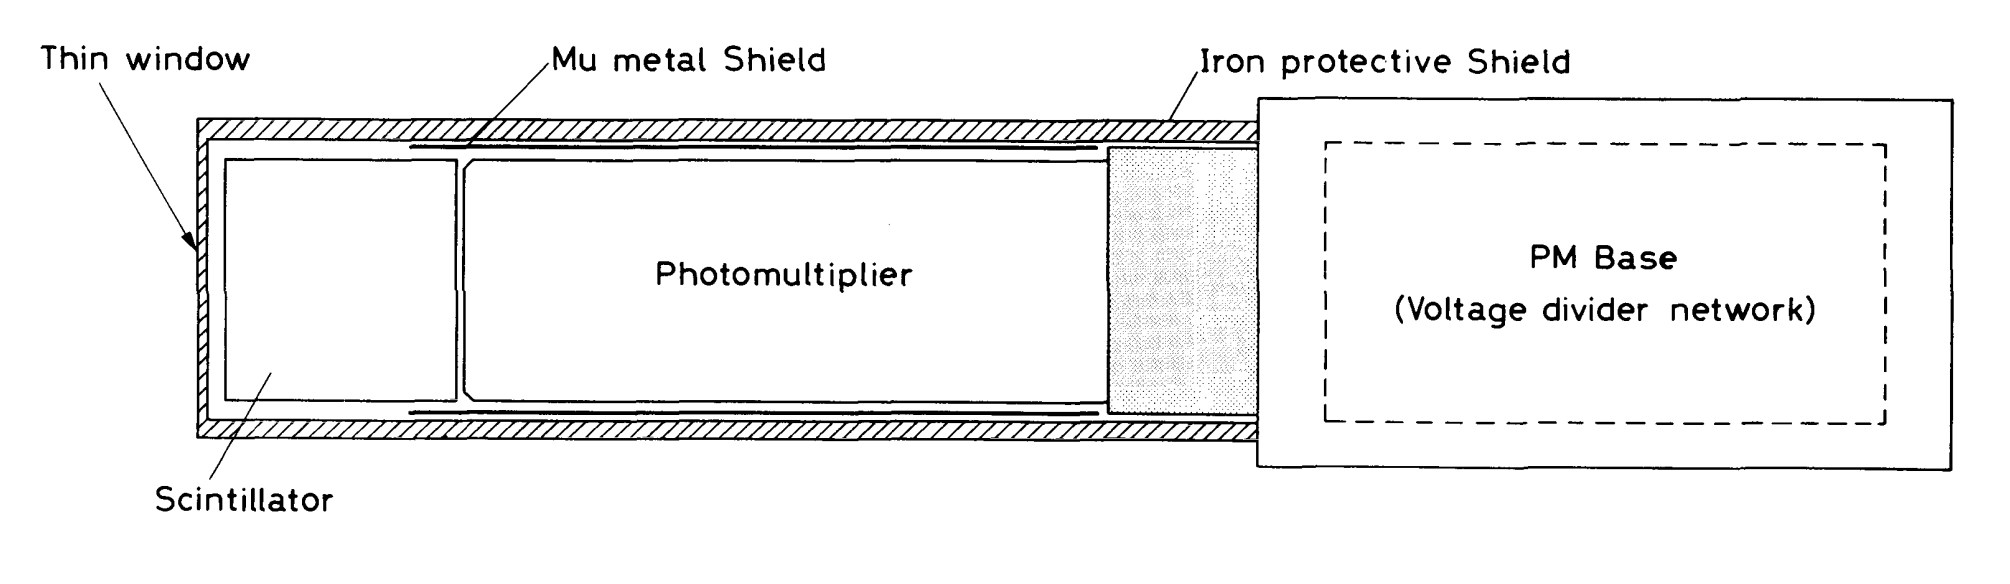
\includegraphics[width=1.1\linewidth]{../Images/Scintillator.png}
    \caption{Schematic diagram of a scintillator~\cite{leo1994techniques}}
    \label{fig:scintillator}
\end{figure}
\begin{figure}[H]
    \centering
    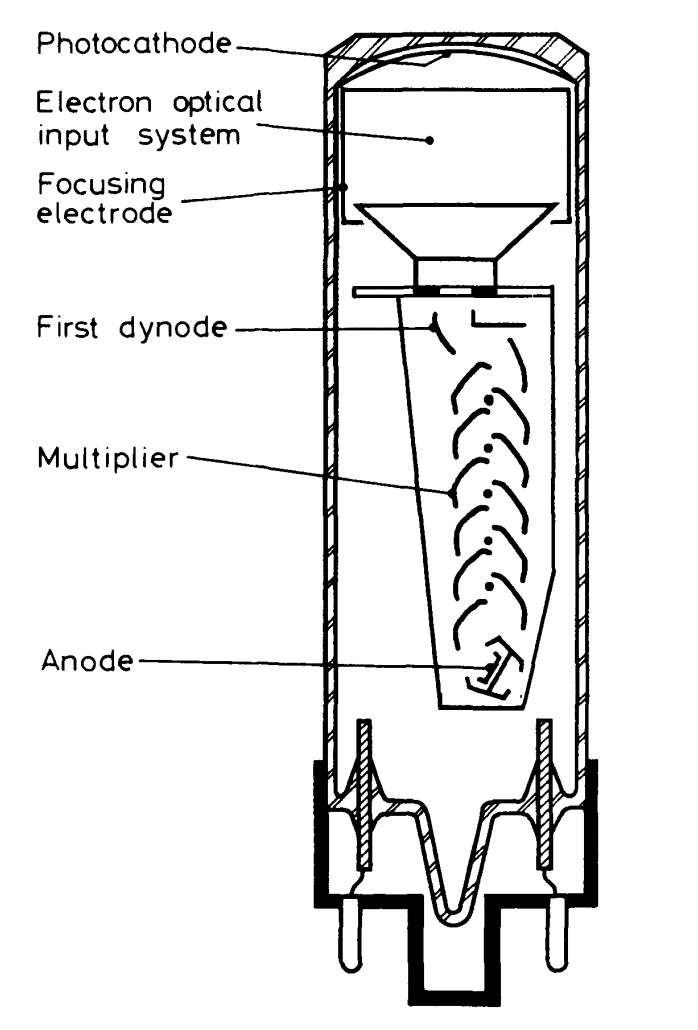
\includegraphics[width=0.5\linewidth]{../Images/Photomultiplier.png}
    \caption{Schematic diagram of a photomultiplier~\cite{leo1994techniques}}
    \label{fig:photomultiplier}
\end{figure}
\end{multicols}

\subsubsection{Single Channel Analyser (SCA)}

An SCA takes in an analog signal and outputs a digital square wave signal, which depends on the amplitude of the input signal. It has an upper and a lower amplitude threshold which can both be adjusted, and any signals falling outside these are blocked.\\

\subsubsection{Multichannel Analyser (MCA)}

Like an SCA, an MCA too takes in analog signals and converts them to a digital output. However, as the name suggests, it is capable of outputting a larger range of digital values (instead of just 1 and 0 like an SCA). It thus has a series of thresholds, like the bins of a histogram, with signals falling into different `bins' producing different digital responses. The MCA also stores these outputs in channel bins reflecting the thresholds, which thus can be used to generate a spectrum showing the different amplitudes it has received as input.\\

While the thresholds of an MCA are set by the manufacturers and cannot be modified like those of an SCA, we can input into an MCA a square wave gate signal, acting as thresholds outside of which the MCA will not record any input signals.\\

\subsubsection{Constant Fraction Discriminator (CFD)}

Two coincident signals with different amplitudes can cause a walk effect in an SCA, where they cross its lower threshold at different times resulting in different, time-delayed outputs for the two. One way to correct this is to use a CFD, which instead of producing a digital signal at the moment an input analog signal crosses a threshold, generates the output at a constant fraction of the peak height, which eliminates any walk effects.\\

The way the CFD works is by splitting an incoming pulse into two. One part is delayed by the time needed for the signal to rise from the chosen constant fraction level to its peak, while the other part is inverted and attenuated by the constant fraction. The two parts are then added together, and the point where the resulting signal has zero amplitude is then at the chosen constant fraction of the signal height.\\

\subsection{$\gamma-\gamma$ cascade and angular correlation}

For a naïve treatment of the directional correlation from a $\gamma-\gamma$ cascade, we begin by first considering a single $\gamma$-transition. Let this transition (of angular momentum $\textbf{L}$) be from an initial nuclear level i to a final nuclear level f, with their spins being $\textbf{I}_i$ and $\textbf{I}_f = \textbf{I}_i - \textbf{L}$ respectively. The quantum numbers of these two levels are thus $I_i, m_i$ and $I_f, m_f$ respectively. The gamma ray has an angular momentum quantum number (or multipolarity) $L$ and a magnetic quantum number $M = m_i-m_f$.\\

For every $\gamma$-transition between some $m_i$ to some $m_f$, there is a directional distribution $F_L^M(\theta)$ ($\theta$ being the angle between the emitted gamma ray and the Z-axis) which is independent of the spins $\textbf{I}_i$ and $\textbf{I}_f$. Since we are generally unable to observe the splitting of the radiation from these different components (as in the Zeeman effect), we generally observe the unresolved line, containing the transitions between every possible pair of magnetic quantum numbers. This has a directional distribution $F_L(\theta)$, to calculate which we need all the $F_L^M(\theta)$, the relative population $P(m_i)$ of each sub-level $m_i$, and the relative transition probability $G(m_i, m_f)$ for each pair of $m_i$ and $m_f$. Then,
$$F_L(\theta) \propto \sum_{m_i,m_f} P(m_i) \ G(m_i,m_f) \ F_L^M(\theta)$$
Using the Clebsch-Gordan coefficients for the quantum numbers $I_i, m_i, I_f, m_f$ allows us to replace the relative transition probability as
$$G(m_i, m_f) = |\langle I_fm_fLM|I_im_i \rangle|^2$$\\

We can now consider a $\gamma-\gamma$ cascade which we will assume happens through the nuclear levels $I_i \rightarrow I \rightarrow I_f$, and emits two gamma-rays of multipolarity $L_1$ and $L_2$. We can set our coordinate axis such that the Z-axis is in the direction of the first gamma-ray's emission. Then, the directional correlation function $W(\theta)$ of the cascade is simply the distribution $F_L(\theta)$ of the second gamma-ray with respect to the Z-axis.\\

The distribution can thus be calculated once each relative probability $P(m)$ for the intermediate sub-levels is known. This is given by the sum of all transitions $m_i \rightarrow m$. Assuming all $m_i$ states are equally populated, we have
$$P(m) \propto \sum_{m_i} G(m_i,m) \ F_{L_1}^{M_1}(\theta=0)$$
A propagating photon can only carry in its direction of motion an angular momentum $\pm h$, and because we had chosen the Z-axis to be along the direction of the first gamma-ray, we can restrict $M_1$ to the values $\pm1$. So, the directional correlation can be calculated as
\begin{align*}
    W(\theta) = F_L(\theta) & \propto \sum_{m,m_f} P(m) \ G(m,m_f) \ F_{L_2}^{M_2}(\theta)\\
    \implies W(\theta) & \propto \sum_{m_i,m,m_f} |\langle I m L_1 \pm1|I_im_i \rangle|^2 \ F_{L_1}^{\pm1}(0) \ |\langle I_f m_f L_2 M_2|I_im_i \rangle|^2 \ F_{L_2}^{M_2}(\theta)\\
\end{align*}

When the gamma-rays emitted in the cascade are both pure (i.e. $L_1$ and $L_2$ have one value each instead of being of a mixed multipole character), the above expression can be simplified to
$$W(\theta) = 1 + A_{22}P_2(\cos\theta) + \ldots + A_{k_{max}k_{max}}P_{k_{max}}(\cos\theta)$$
where $P_n$ are the Legendre polynomials, and
$$k_{max} = \min(2I, 2L_1, 2L_2)$$

\subsection{Decay Scheme of $^{60}$Co}

\begin{figure}[H]
    \centering
    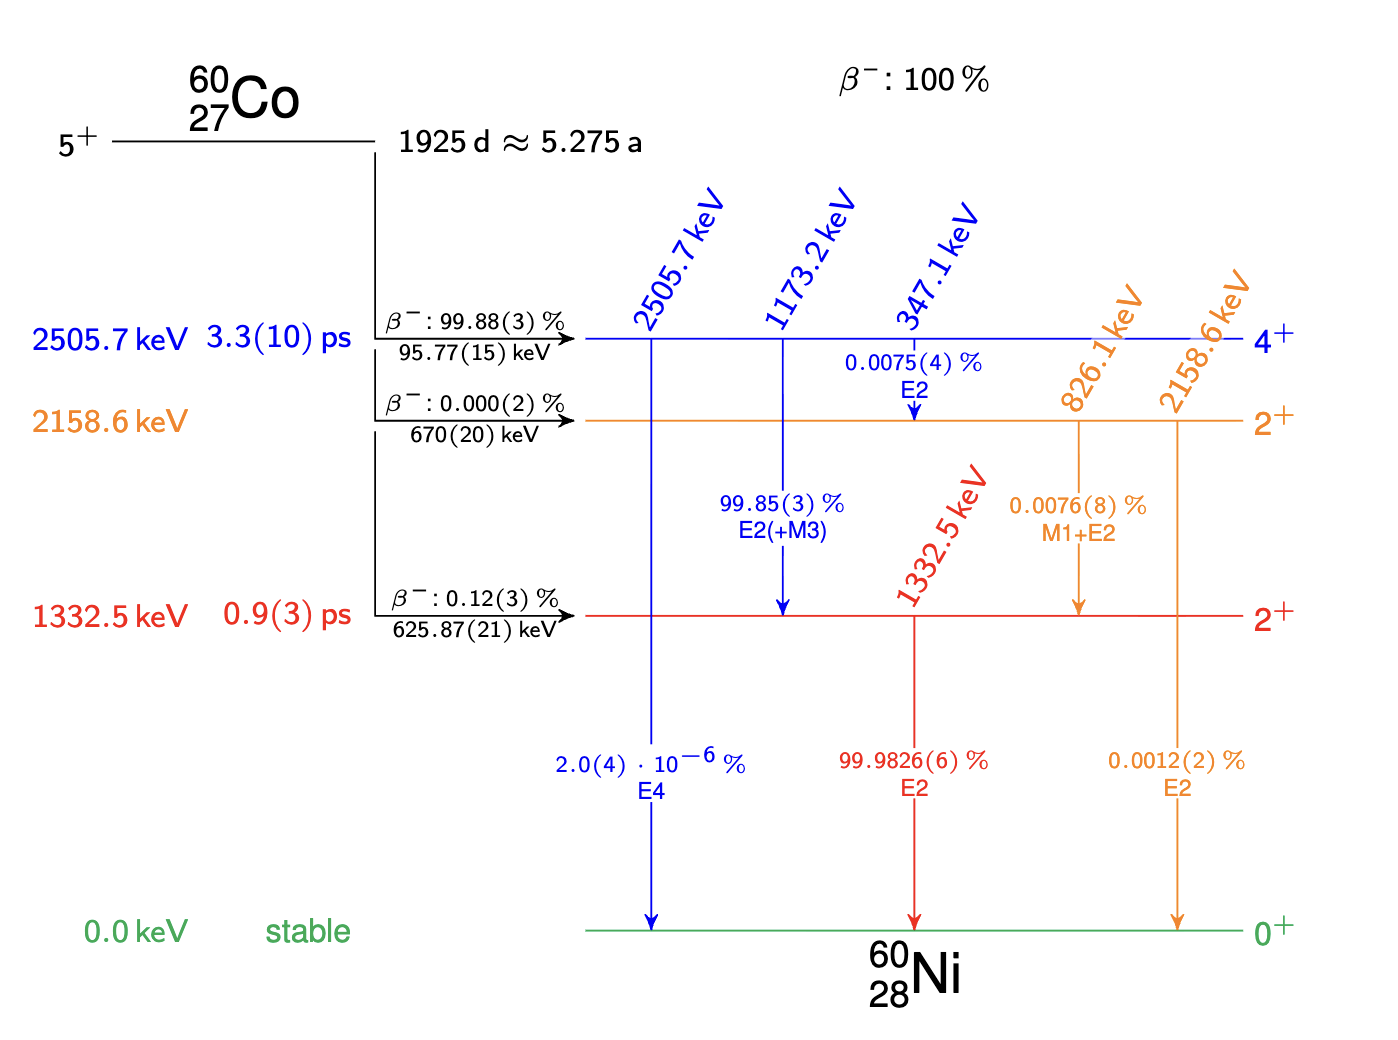
\includegraphics[width=0.6\linewidth]{../Images/Decay Scheme.png}
    \caption{Decay Scheme of $^{60}$Co~\cite{Rosinsky2022}}
    \label{fig:decay}
\end{figure}

As can be seen from the decay scheme in Fig. \ref{fig:decay}, $^{60}$Co decays via a $\gamma-\gamma$ cascade into the stable $^{60}$Ni, which has 28 protons and 32 neutrons. (Though there are multiple ways in which the decay occurs, the transitions from the $2505.7\,$keV to the $1332.5\,$keV and then to the ground state are most predominant.) Such an `even-even' nucleus is useful for angular correlation observations of the cascade. The nucleus presumably has a spin 0 in its ground state and hence the second $\gamma$-transition must be pure. Only the first $\gamma$-transition can be mixed.\\

Experimentally, this $\gamma-\gamma$ cascade has been shown to occur between spins 4, 2, and 0, and the corresponding directional correlational function has been calculated to be of the form
$$W(\theta) = 1 + 0.1020P_2(\cos\theta) + 0.0091P_4(\cos\theta)$$\\

\begin{figure}[H]
    \centering
    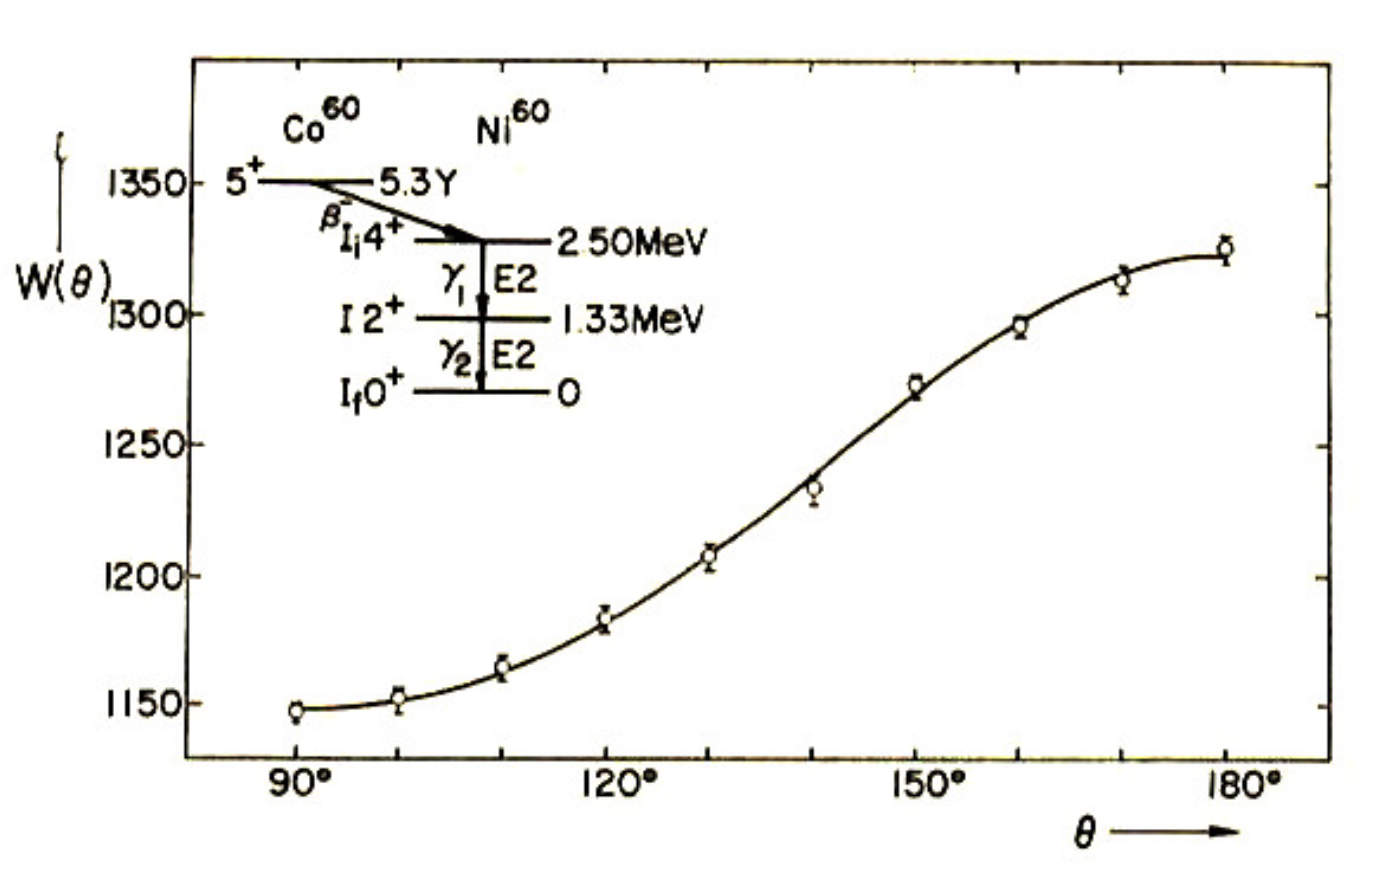
\includegraphics[width=0.6\linewidth]{../Images/Theory Distribution.png}
    \caption{Experimentally obtained directional correlation distribution of the $^{60}$Co to $^{60}$Ni cascade\cite{Steffen}. The solid line is the theoretically determined function $W(\theta)$~\cite{siegbahn}}
    \label{fig:theoryW}
\end{figure}
